\section[Introdução]{Introdução}

O projeto Programa Manejo de Estresse foi pensado e apresentado para nós pelas stakeholders Daiana C. Tech e Meri Fátima Demski (Fundadoras e CEOs da Startup Lumiar Serviços Tenológicos Ltda.) e supervisionado pelo professor orientador Michael da Cost Móra durante o semestre de 2025/1.

O objetivo do projeto é a criação de uma plataforma onde onde seja possível o usuário realizar treinamentos que auxiliam os usuários a obter um melhor controle sobre o estresse que passam durante seu dia-a-dia. Isso é feito através de exercícios de auto controle e reflexão.

\begin{figure}[H]
    \centering
    \small
    \caption{Time Projeto Manejo de Estresse}
    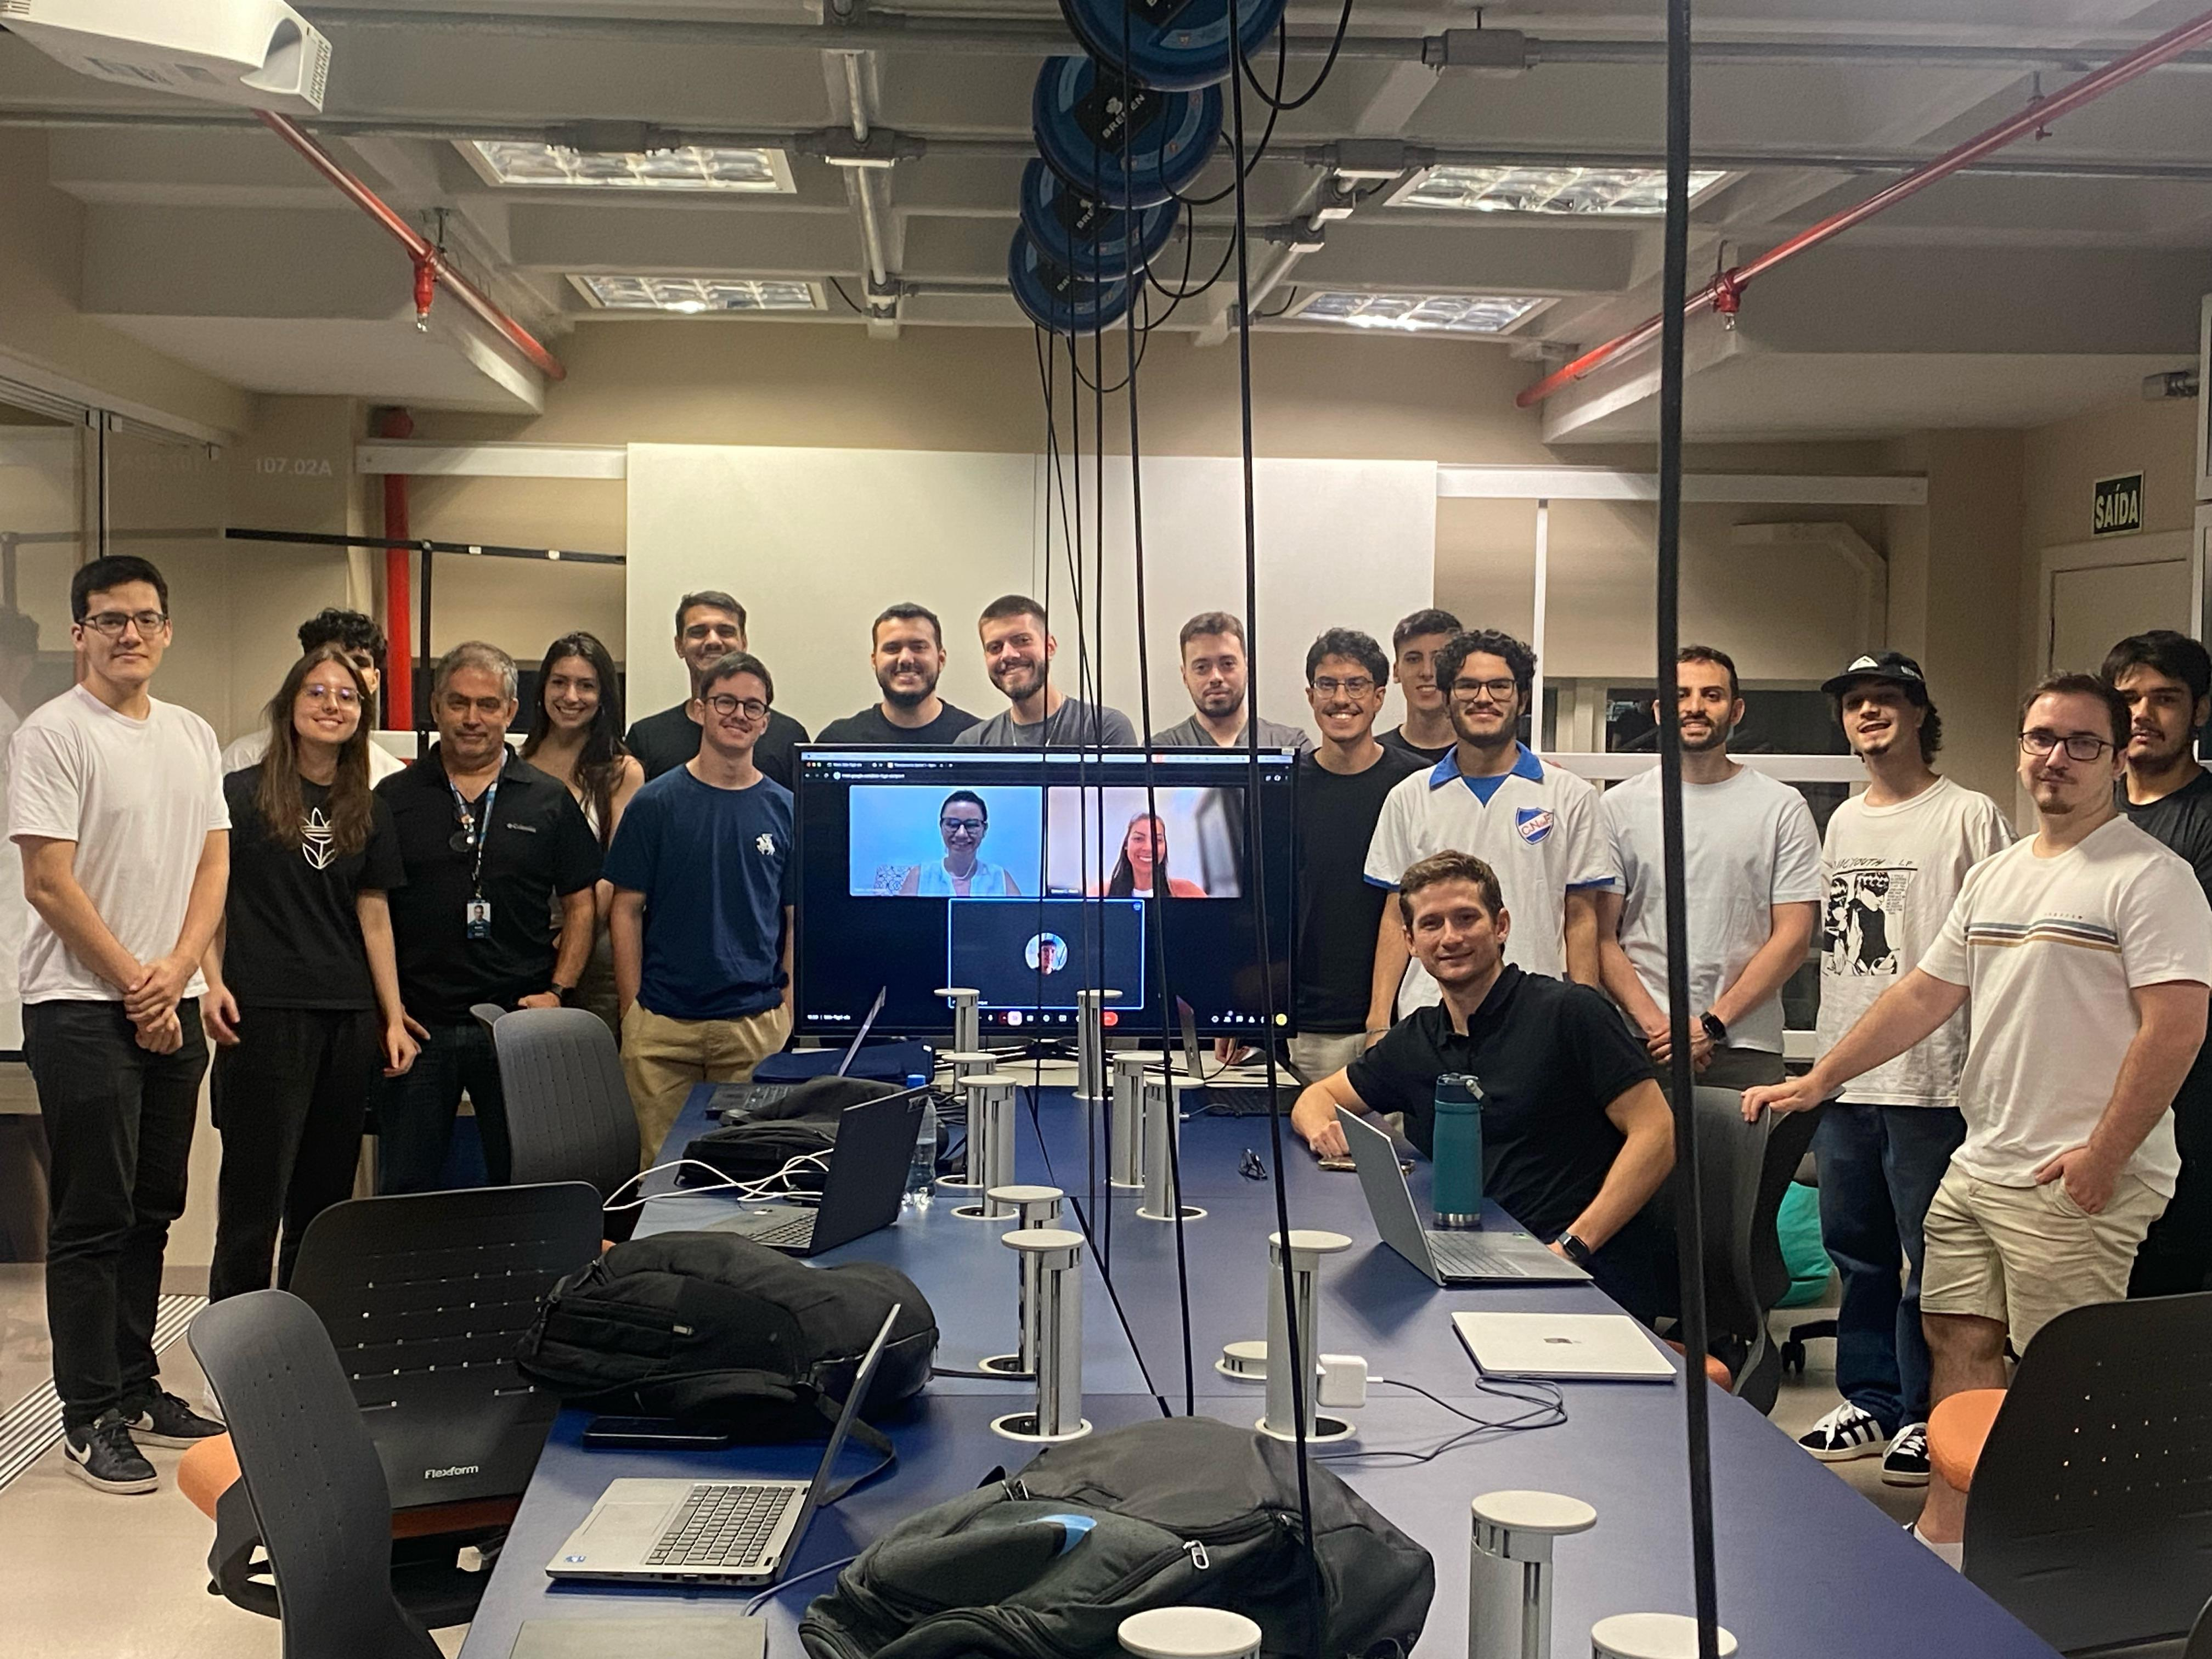
\includegraphics[width=1\linewidth]{conteudo//4 - ages III//conteudo//figures//foto-time.jpg}
    Fonte: https://tools.ages.pucrs.br/treinamentoAutoguiado/wiki/-/tree/main
\end{figure}